
\documentclass[a4paper,11pt]{article}
\usepackage[a4paper, margin=8em]{geometry}

% usa i pacchetti per la scrittura in italiano
\usepackage[french,italian]{babel}
\usepackage[T1]{fontenc}
\usepackage[utf8]{inputenc}
\frenchspacing 

% usa i pacchetti per la formattazione matematica
\usepackage{amsmath, amssymb, amsthm, amsfonts}

% usa altri pacchetti
\usepackage{gensymb}
\usepackage{hyperref}
\usepackage{standalone}

% imposta il titolo
\title{Appunti Calcolo Numerico}
\author{Luca Seggiani}
\date{2025}

% disegni
\usepackage{pgfplots}
\pgfplotsset{width=10cm,compat=1.9}

% imposta lo stile
% usa helvetica
\usepackage[scaled]{helvet}
% usa palatino
\usepackage{palatino}
% usa un font monospazio guardabile
\usepackage{lmodern}

% tikz in sans
\tikzset{every picture/.style={/utils/exec={\sffamily}}}

\renewcommand{\rmdefault}{ppl}
\renewcommand{\sfdefault}{phv}
\renewcommand{\ttdefault}{lmtt}

% circuiti
\usepackage{circuitikz}
\usetikzlibrary{babel}

% disponi il titolo
\makeatletter
\renewcommand{\maketitle} {
	\begin{center} 
		\begin{minipage}[t]{.8\textwidth}
			\textsf{\huge\bfseries \@title} 
		\end{minipage}%
		\begin{minipage}[t]{.2\textwidth}
			\raggedleft \vspace{-1.65em}
			\textsf{\small \@author} \vfill
			\textsf{\small \@date}
		\end{minipage}
		\par
	\end{center}

	\thispagestyle{empty}
	\pagestyle{fancy}
}
\makeatother

% disponi teoremi
\usepackage{tcolorbox}
\newtcolorbox[auto counter, number within=section]{theorem}[2][]{%
	colback=blue!10, 
	colframe=blue!40!black, 
	sharp corners=northwest,
	fonttitle=\sffamily\bfseries, 
	title=Teorema~\thetcbcounter: #2, 
	#1
}

% disponi definizioni
\newtcolorbox[auto counter, number within=section]{definition}[2][]{%
	colback=red!10,
	colframe=red!40!black,
	sharp corners=northwest,
	fonttitle=\sffamily\bfseries,
	title=Definizione~\thetcbcounter: #2,
	#1
}

% disponi problemi
\newtcolorbox[auto counter, number within=section]{problem}[2][]{%
	colback=green!10,
	colframe=green!40!black,
	sharp corners=northwest,
	fonttitle=\sffamily\bfseries,
	title=Problema~\thetcbcounter: #2,
	#1
}

% disponi codice
\usepackage{listings}
\usepackage[table]{xcolor}

\definecolor{codegreen}{rgb}{0,0.6,0}
\definecolor{codegray}{rgb}{0.5,0.5,0.5}
\definecolor{codepurple}{rgb}{0.58,0,0.82}
\definecolor{backcolour}{rgb}{0.95,0.95,0.92}

\lstdefinestyle{codestyle}{
		backgroundcolor=\color{black!5}, 
		commentstyle=\color{codegreen},
		keywordstyle=\bfseries\color{magenta},
		numberstyle=\sffamily\tiny\color{black!60},
		stringstyle=\color{green!50!black},
		basicstyle=\ttfamily\footnotesize,
		breakatwhitespace=false,         
		breaklines=true,                 
		captionpos=b,                    
		keepspaces=true,                 
		numbers=left,                    
		numbersep=5pt,                  
		showspaces=false,                
		showstringspaces=false,
		showtabs=false,                  
		tabsize=2
}

\lstdefinestyle{shellstyle}{
		backgroundcolor=\color{black!5}, 
		basicstyle=\ttfamily\footnotesize\color{black}, 
		commentstyle=\color{black}, 
		keywordstyle=\color{black},
		numberstyle=\color{black!5},
		stringstyle=\color{black}, 
		showspaces=false,
		showstringspaces=false, 
		showtabs=false, 
		tabsize=2, 
		numbers=none, 
		breaklines=true
}

\lstdefinelanguage{javascript}{
	keywords={typeof, new, true, false, catch, function, return, null, catch, switch, var, if, in, while, do, else, case, break},
	keywordstyle=\color{blue}\bfseries,
	ndkeywords={class, export, boolean, throw, implements, import, this},
	ndkeywordstyle=\color{darkgray}\bfseries,
	identifierstyle=\color{black},
	sensitive=false,
	comment=[l]{//},
	morecomment=[s]{/*}{*/},
	commentstyle=\color{purple}\ttfamily,
	stringstyle=\color{red}\ttfamily,
	morestring=[b]',
	morestring=[b]"
}

% disponi sezioni
\usepackage{titlesec}

\titleformat{\section}
	{\sffamily\Large\bfseries} 
	{\thesection}{1em}{} 
\titleformat{\subsection}
	{\sffamily\large\bfseries}   
	{\thesubsection}{1em}{} 
\titleformat{\subsubsection}
	{\sffamily\normalsize\bfseries} 
	{\thesubsubsection}{1em}{}

% disponi alberi
\usepackage{forest}

\forestset{
	rectstyle/.style={
		for tree={rectangle,draw,font=\large\sffamily}
	},
	roundstyle/.style={
		for tree={circle,draw,font=\large}
	}
}

% disponi algoritmi
\usepackage{algorithm}
\usepackage{algorithmic}
\makeatletter
\renewcommand{\ALG@name}{Algoritmo}
\makeatother

% disponi numeri di pagina
\usepackage{fancyhdr}
\fancyhf{} 
\fancyfoot[L]{\sffamily{\thepage}}

\makeatletter
\fancyhead[L]{\raisebox{1ex}[0pt][0pt]{\sffamily{\@title \ \@date}}} 
\fancyhead[R]{\raisebox{1ex}[0pt][0pt]{\sffamily{\@author}}}
\makeatother

\begin{document}

% sezione (data)
\section{Lezione del 05-05-25}

% stili pagina
\thispagestyle{empty}
\pagestyle{fancy}

% testo
Continuiamo la trattazione dell'approssimazione di integrali attraverso le formule di quadratura interpolatorie.
Un problema che avevamo fino adesso è che se $h$ è grande, allora $E_n(f)$ è grande per qualche termine proporzionale a $h^d$, dove $d$ è il grado dell'errore.

Un'idea potrebbe essere di aumentare $n$, quindi aumentare i punti campionati per ridurre il passo $h$, ma come abbiamo visto questo è instabile (risente di fenomeni simili al fenomeno di Runge).

\subsubsection{Formule di Newton-Cotes generalizzate}
Decidiamo quindi di spezzare l'integrale su sottointervalli, e in ciascuno di essi applicare una formula di quadratura.
Questo metodo ci porterà alle formule di Newton-Cotes \textbf{generalizzate}, anche dette \textit{composite}.

Quindi, posto ad esempio un certo intervallo $[a, b]$ contenente i punti ordinati $c, d, e$, dividiamo l'integrale:
$$
\int_a^b f(x) \, dx = \int_a^c f(x) \, dx + \int_c^d f(x) \, dx + \int_d^e f(x) \, dx + \int_e^b f(x) \, dx
$$
e si applica la formula di quadratura ad ogni sottointervallo, sommando.

Più formalmente, avremo che si divide $[a, b]$ in $L$ sottointervalli equispaziati, con:
$$
x_0 = a, \quad x_1 = x_0 + \frac{b - a}{L}, \quad ..., \quad x_L = b
$$
e si divide l'integrale come:
$$
\int_a^b f(x) \, dx = \sum_{i = 1}^L \int_{x_{i - 1}}^{x_i} f(x) \, dx
$$
In ogni intervallo $[x_{i - 1}, x_i]$ si applica quindi una formula di Newton Cotes con $n + 1$ nodi.

Avremo quindi bisogno, in ogni sottointervallo, di:
$$
n + 1 - 2 = n - 1
$$ 
nodi aggiuntivi oltre agli estremi dell'intervallo per poter applicare la formula di quadratura $J_n(f)$.
Il numero di nodi totali dovrà quindi essere:
$$
L + 1 + (n - 1) \cdot L = nL + 1
$$

Osserviamo che il numero di nodi corrisponde al numero di valutazioni di $f$, e quindi in genere è un'indicazione del costo computazionale di una formula. 

\subsubsection{Esempio: formula dei trapezi generalizzata}
Prendiamo la forma che otteniamo per $n = 1$:
$$
\int_a^b f(x) \, dx \approx \sum_{i = 1}^L \frac{b - a}{2L} \left( f(x_{i - 1}) + f(x_i) \right) = \frac{b - a}{2L} \sum_{i = 1}^L \left( f(x_{i - 1}) + f(x_i) \right)
$$
$$
= \frac{b - a}{2L} \left( f(x_0) + 2 \sum_{i = 1}^{L - 1} f(x_i) + f(x_L) \right) = J_1^{(G)} (f)
$$

\subsubsection{Esempio: formula di Cavalieri-Simspon}
Vediamo quindi la generalizzazione della formula di Cavalieri, cioè ciò che otteniamo per $n = 2$:
$$
\int_a^b f(x) \, dx \approx \sum_{i = 1}^L \frac{b - a}{6L} \left( f(x_{i - 1}) + 4 f \left( \frac{x_{i - 1} + x_i}{2} \right) + f(x_i) \right)
$$
$$
= \frac{b - a}{6L} \left( f(x_0) + 2 \sum_{i = 1}^{L-1} f(x_i) + 4 \sum_{i = 1}^{L} f\left( \frac{x_{i - 1} + x_i}{2} \right) + f(x_L) \right) = J_2^{(G)} (f)
$$

\subsubsection{Errore nelle formule generalizzate}
In ogni intervallo della forma $[x_{i - 1}, x_i]$ conosciamo l'errore, che è quello della formula di Newton-Cotes che stiamo utilizzando:
$$
e \cdot h^d \cdot f^{(d - 1)} (\varepsilon), \quad f \in C^{(d - 1)} ([a, b])
$$
L'errore sulla formula totale $J_n^{(G)}(f)$ sarà quindi:
$$
E_n^{(G)} (f) = I(f) - J_n^{(G)} (f) = \sum_{i = 1}^L c \cdot h^d \cdot f^{(d - 1)}(\varepsilon_i), \quad \varepsilon_i \in [x_{i - 1}, x_i]
$$
Vediamo quindi che l'unico termine dipendente dall'intervallo è $f^{(d - 1)} (\varepsilon)$, per cui possiamo dire:
$$
= \sum_{i = 1}^L c \cdot h^d \cdot L \frac{f^{(d - 1)}(\varepsilon_i)}{L} = c h^dL \cdot f^{(d - 1)} (\varepsilon), \quad \varepsilon \in [a, b]
$$
sfruttando il teorema della media integrale.

Abbiamo quindi gli errori:
\begin{itemize}
	\item \textbf{Formula dei trapezi:}
		$$
		E_1^{(G)}(f) = -\frac{(b - a)^3}{12L^2} \cdot f''(\varepsilon)
		$$
	\item \textbf{Formula di Cavalieri-Simpson:}
		$$
		E_2^{(G)}(f) = -\frac{(b - a)^5}{2880L^4} \cdot f^{(4)} (\varepsilon), \quad \varepsilon \in [a, b]
		$$
\end{itemize}
e il caso generale:
$$
E_n^{(G)} (f) =
\begin{cases}
	c_n \cdot \frac{(b - a)^{n + 2}}{L^{n + 1}} \cdot f^{(n + 1)} (\varepsilon), \quad n \text{ dispari} \\
	c_n \cdot \frac{(b - a)^{n + 3}}{L^{n + 2}} \cdot f^{(n + 2)} (\varepsilon), \quad n \text{ pari} \\
\end{cases}
$$

\subsection{Formule di quadratura sulle derivate}
Potremmo considerare formule di quadratura che coinvolgono le derivate di $f$.
Si possono quindi generalizzare i concetti di grado di precisione, scelta dei nodi e pesi ottimali anche per formule di quadratura del tipo:
$$
\int_a^b f(x) \rho(x) \, dx = \sum_{i = 0}^{n_1} f(x_i) + \sum_{i = 0}^{n_2} f'(y_i) + \sum_{i = 0}^{n_3} f''(z_i)
$$
chiaramente restringendo l'applicazione delle formule a funzioni sufficientemente derivabili.

Vediamo ad esempio come trovare i pesi ottimi per l'approssimazione con:
$$
\int_0^1 f(x) \, dx = I(f) \approx a_1 f(0) + a_2 f' \left( \frac{1}{3} \right) + a_3 f' \left( \frac{2}{3} \right) + f(1)
$$
sull'intervallo $[a, b] = [0, 1]$.

Imponendo errore nullo ai primi 4 gradi si otterrà:
\[
	\begin{cases}
		E_1(1)= 0 \\
		E_1(x)= 0 \\
		E_1(x^2)= 0 \\
		E_1(x^3)= 0 
	\end{cases}
	\implies
	\begin{cases}
		\int_0^1 1 \, dx = 1 = a_1 + a_4 \\ 
		\int_0^1 x \, dx = \frac{1}{2} = a_2 + a_3 + a_4 \\
		\int_0^1 x^2 \, dx = \frac{1}{3} = \frac{2}{3} a_2 + \frac{4}{3} a_3 + a_4 \\
		\int_0^1 x^3 \, dx = \frac{1}{4} = \frac{1}{3} a_2 + \frac{4}{3} a_3 + a_4
	\end{cases}
\]
Ricaviamo allora dalle prime 3:
\[
	\begin{cases}
		a_4 = 1 - a_1 \\
		a_2 = \frac{1}{2} - a_3 - a_4 \\ 
		a_3 = \frac{3}{4} \left( \frac{1}{3} - \frac{2}{3} a_2 - a_4 \right) = \frac{1}{4} - \frac{1}{2} a_2 - \frac{3}{4} a_4
\end{cases}
\]
da cui sostituendo ulteriormente:
\[
	\begin{cases}
		a_4 = 1 - a_1 \\ 
		a_2 = \frac{1}{2} + \frac{1}{2} a_4 - a_4 = \frac{1}{2} - \frac{1}{2}a_4 \\ 
		a_3 = \frac{1}{4} - \frac{1}{2} \left( \frac{1}{2} - a_3 - a_4 \right) - \frac{3}{4} a_4 = \frac{1}{2} a_3 - \frac{1}{4}a_4
	\end{cases}
\]
sostituendo tutto nella quarta si ha:
$$
\frac{1}{4} = \frac{1}{3} \left( \frac{1}{2} - \frac{1}{2} a_4 \right) + \frac{4}{3} \cdot - \frac{1}{2} a_4 + a_4 = \frac{1}{6} + \frac{1}{6} a_4 \implies a_4 \frac{1}{2} 
$$
da cui immediatamente:
$$
a_1 = \frac{1}{2}, \quad
a_2 = \frac{1}{4}, \quad
a_3 = -\frac{1}{4}, \quad
a_4 = \frac{1}{2}, \quad
$$
da cui:
$$
J_3(f) = \frac{f(0)}{2} + \frac{f' \left( \frac{1}{3} \right)}{4} - \frac{f'' \left( \frac{2}{3} \right)}{4} + \frac{f(1)}{2}
$$

Per determinare il grado di precisione vediamo l'errore per $x^4$:
$$
E_3(x^4) = \int_0^1 x^4 \, dx - \left( \frac{1}{2} \cdot 0 + \frac{1}{4} \cdot 4 \cdot \left( \frac{1}{3} \right)^3 - \frac{1}{4} \cdot 4 \cdot \left( \frac{2}{3} \right)^3 + \frac{1}{2} \right) = \frac{1}{5} - \left( \frac{1}{27} - \frac{8}{27} + \frac{1}{2} \right) = \frac{1}{5} - \frac{13}{54} \neq 0
$$
da cui il grado di precisione è esattamente 3.

\subsection{Implementazione MATLAB dei metodi di approssimazione di integrali}
Possiamo quindi implementare quanto abbiamo studiato finora in funzioni MATLAB che ci permettano di approssimare gli integrali di certi function handle su dati intervalli.

Definiamo in particolare una funzione di approssimazione composita di grado 1 (metodo dei trapezi) e 2 (metodo di Cavalieri-Simpson).

\subsubsection{Implementazione MATLAB del metodo dei trapezi}
Potremo implementare direttamente la funzione descritta in 18.0.2, con un pò di logica aggiuntiva per tracciare un grafico delle rette approssimazione, come:

\lstset{language=MATLAB,style=codestyle}
\lstinputlisting{../code/matlab/trapez_int.m}

\subsubsection{Implementazione MATLAB del metodo di Cavalieri-Simpson}
Anche qui otremo implementare direttamente la funzione descritta in 18.0.3, con un pò di logica aggiuntiva per tracciare un grafico delle parabole di approssimazione, come:

\lstset{language=MATLAB,style=codestyle}
\lstinputlisting{../code/matlab/simpson_int.m}
dove notiamo che manteniamo esplicitamente i punti intermedi separati dai punti estremi degli intervalli di integrazione, ergo $L$ determina il numero di intervalli di integrazione.

\par\medskip

Potremo quindi provare gli algoritmi, ad esempio sulla funzione:
$$
f(x) = \sin\left(x\right)+\tan\left(\frac{x}{15}\right)+e^{-x} 
$$
sull'intervallo $[a, b]] = [0, 15]$.

Iniziamo col definire le variabili e un valore di \textit{ground truth}, usando la \lstinline|integral()| fornita da MATLAB:
\begin{lstlisting}[language=MATLAB, style=codestyle]	
>> f = @(x) sin(x) .* tan(x / 15) + exp(-x); % definiamo f
>> a = 0; b = 15;
>> i = integral(f, a, b)

i =

    2.2912
\end{lstlisting}

Potremo quindi provare il metodo dei trapezi come:
\begin{lstlisting}[language=MATLAB, style=codestyle]	
>> jt = trapez_int(f, a, b, 10)

jt =

    2.2734
\end{lstlisting}

Da cui otteniamo un valore di $i - j_t \approx 0.0178$, e il grafico:
\begin{center}
	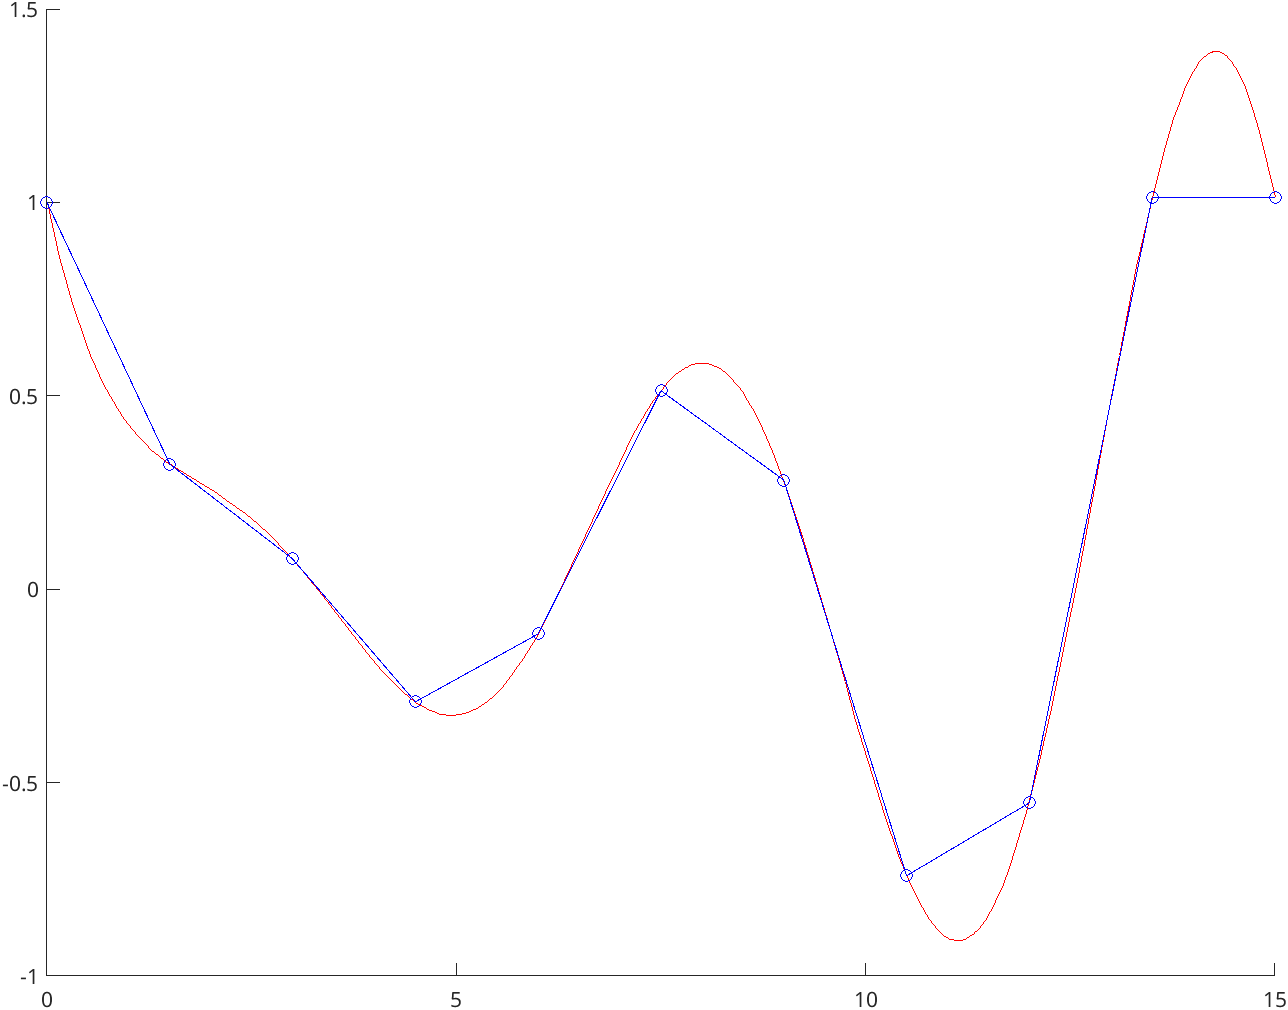
\includegraphics{../figures/matlab_trapez_int.png}
\end{center}

Vediamo quindi se l'approssimazione col metodo di Cavalieri-Simpson è più accurata:
\begin{lstlisting}[language=MATLAB, style=codestyle]	
>> js = simpson_int(f, a, b, 10)

js =

    2.2940
\end{lstlisting}

\newpage
In questo caso otteniamo il valore $i - j_s \approx -0.0028$, e il grafico:
\begin{center}
	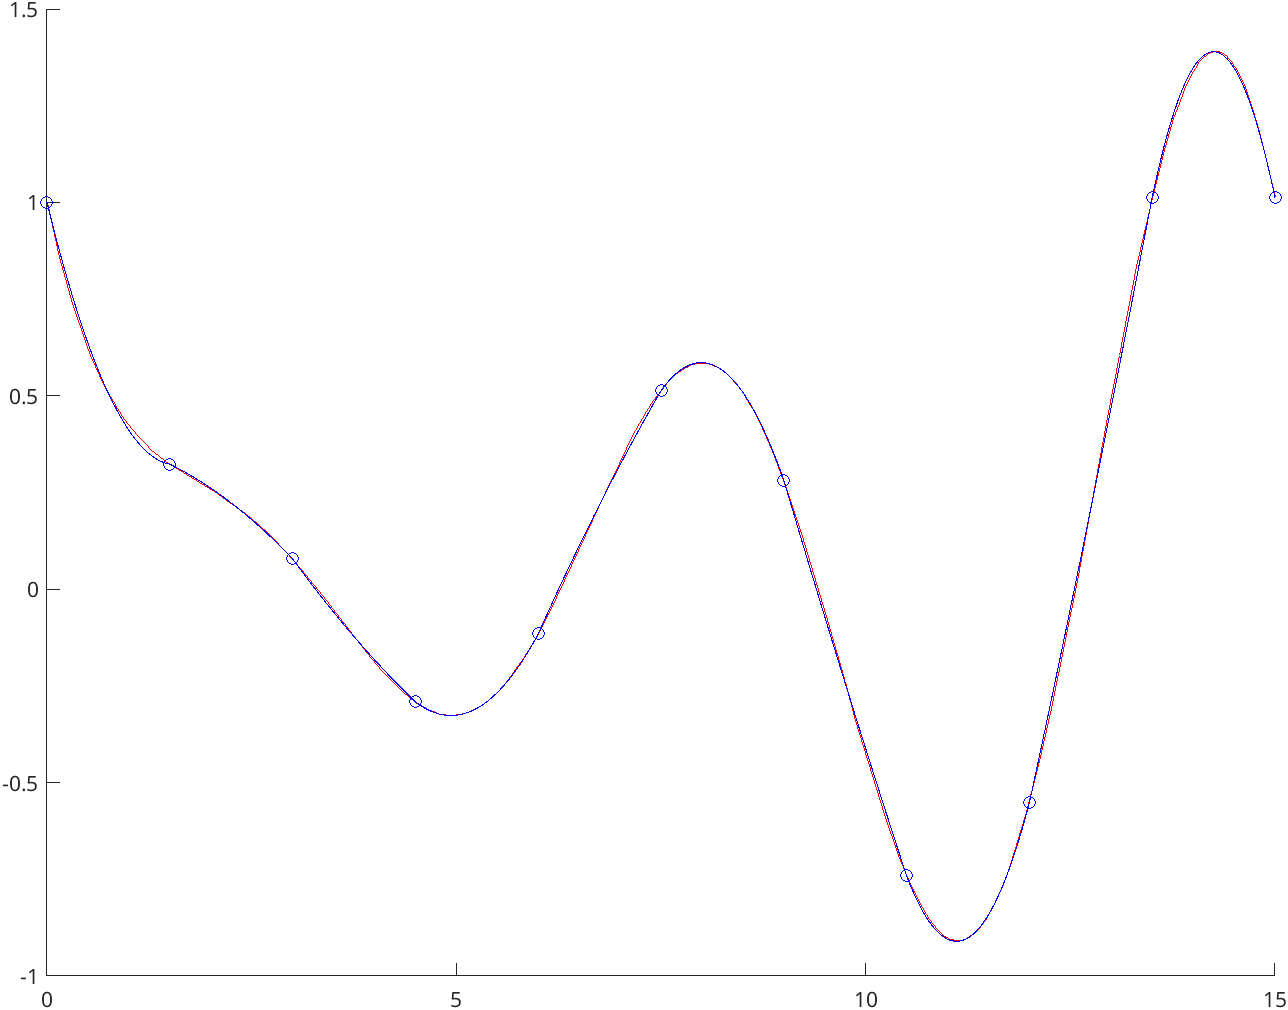
\includegraphics{../figures/matlab_simpson_int.png}
\end{center}
cioè notiamo che sia il grafico che l'appossimazione integrale sono molto pià vicini alla funzione originale.

\end{document}
